\documentclass[twoside]{article}
\input{ISC18-english.sty}
%%%%%%%%%%%%%%%%%%%%%%%%%%%%  Make sure to compile twice for proper cross-references. %%%%%%%%%%%%%%%%%%%%%%%
%%%%%%% For proper display of references, compile the document twice. %%%%%%%%%%%%%%%%%%%%% 
%%%%%%%%%%%%%%% If using TeX Live, compile using pdflatex command %%%%%%%%%%%%%%%%%%%%%%%
\begin{document}
\thispagestyle{empty}
%%%%%%%%%%%%%%%%% Article title header  %%%%%%%%%%%%%%%%%%%%
\fancyhead[LE]{CDF Inference under JPS}
%%%%%%%%%%%%%%%%% Article authors header   %%%%%%%%%%%%%%%%%%%%
\fancyhead[RO]{}Azizi Kouhanestani, Zamanzade and Goli
\begin{center}
{
\includegraphics [height=25mm, width=150.3mm] {Images/isc18E}} \\
\vspace*{-1.8cm}
%\begin{center}
%\color{blue} 
%{\hspace{0.1cm}\rule{\textwidth}{1mm}}\\
%\end{center}
\vspace*{4cm}
%%%%%%%%%%%%%%%%% Article title  %%%%%%%%%%%%%%%%%%%%
{\Large \bf A Review of Smooth Estimation of the Cumulative Distribution Function under Judgment Post Stratification
}\\
%%%%%%%%%%%%%%%%% Article authors and affiliations %%%%%%%%%%%%%%%%%%%%
{\bf
Azizi Kouhanestani, M.$^1$, Zamanzade, E.$^2$, Goli, S.$^1$ \footnote[2]{{\bf Corresponding Author:} {\tt  e.zamanzade@sci.ui.ac.ir }} \\$^1$ Department of Mathematical Sciences, Isfahan University of Technology, Isfahan, Iran \\
$^2$ Department of Statistics, Faculty of Mathematics and Statistics, University of Isfahan, Isfahan, Iran}
\end{center}
\rule{\textwidth}{0.2mm}\\
%%%%%%%%%%%%%%%%% Article abstract  %%%%%%%%%%%%%%%%%%%%
\noindent{\bf Abstract:}\\
This paper provides a review of smooth estimation methods for the cumulative distribution function (CDF) under the judgment post stratification (JPS) sampling scheme. Particular attention is devoted to a general class of CDF estimators that encompasses both empirical and kernel-based estimators. The main finite-sample and asymptotic properties of these estimators are summarized and discussed.
To further illustrate their performance, an extended Monte Carlo simulation study is conducted to compare the kernel distribution function (KDF) estimator under JPS with its counterpart based on simple random sampling (SRS). The comparison considers a range of sample sizes, set sizes, and ranking qualities. The findings demonstrate that incorporating ranking information through the JPS design can lead to considerable efficiency gains relative to SRS across a broad spectrum of settings.


%In this work, we discuss a general class of estimators for the cumulative distribution function (CDF) based on judgment post stratification  (JPS)   sampling scheme, which includes both empirical and kernel distribution functions. 
%  Specifically, we obtain the expectation of the estimators in this class and show that they are asymptotically more efficient than their competitors in simple random sampling (SRS), as long as the rankings are better than random guessing. We find a mild condition that is necessary and sufficient for them to be asymptotically unbiased. We also prove that  given the same condition, the estimators in this class are strongly uniformly consistent estimators of the true CDF,  and converge in distribution to a normal distribution when the sample size approaches infinity.
% We then focus on the kernel distribution function (KDF)  in the JPS design and  obtain the optimal bandwidth. 
%The finite-sample and asymptotic properties of these estimators are presented and discussed.
% We also carry out a comprehensive Monte Carlo simulation to compare the performance of the KDF in the JPS design for different choices of sample size, set size, ranking quality, parent distribution, kernel function, as well as both perfect and imperfect rankings set-ups, with its counterpart in the SRS design. We find that the JPS estimator dramatically improves the efficiency of the KDF compared to its SRS competitor across a wide range of the settings.
 % Finally, we apply the described procedure to a real dataset from a medical context to show its usefulness and applicability in practice.
 
\noindent{\bf Keywords:} 
Nonparametric estimation, Monte Carlo simulation, Judgment ranking, and  Statistical inference \\
\noindent{\bf Mathematics Subject Classification (2020):} $\rm 62D05$, $\rm 62G05$. \\
\hspace{1cm}\rule{\textwidth}{0.2mm}\\
%%%%%%%%%%%%%%
\raggedbottom
\section{Introduction}
Judgment post stratification (JPS) sampling, proposed by \cite{maceachern2004judgement}, is a rank-based sampling design that utilizes  ranking information to improve the efficiency of statistical inference. This sampling scheme is particularly useful in studies where accurate measurement of the variable of interest $(X)$ is difficult, expensive, or time-consuming, while ranking the sampling units can be performed easily and at a relatively low cost. Such situations frequently arise in ecological, medical, and environmental research.
%RSS was  first suggested  by  \citet{mcintyre1952method}. To obtain an RSS sample of size $n$, one first determines the value of $H$ and a vector $ \mathbf{N}=(N_1, \ldots, N_H)$,  where $H$  is called the set size and $ \mathbf{N}$ is called the vector of post strata sample sizes, such that   $N_r$ represents the count of units with rank $r$ that need to be chosen for accurate quantification, ensuring that the sum of all $N_r$ values from $r=1$ to $H$ is equal to $n$.
%He/She then draws asn SRS sample of size $n\times H$ from the population of interest and randomly divides it into $n$   samples of size $H$. In the next step,  each SRS sample of size $H$ is ranked in increasing magnitude without actual measurement.
%Lastly, from the $N_r$ ranked samples of size $H$, units with judgment rank $r$ are marked for accurate quantification ($r=1,  \ldots, H$). If $ N_1= \ldots=N_H$, the sampling scheme is called balanced RSS.
%The term judgment rank  is employed to emphasize that the ranking process relies on personal judgment, visual assessment, or an auxiliary variable that strongly correlates with the variable of interest.
% Hence, it may not be precise and may have some errors, which is called imperfect ranking. The best situation is perfect  ranking, in which there is no error in the mechanism of ranking and thus judgment ranks coincide with the true ones.
%After the introduction of RSS, it was studied in much research.  \citet{takahasi1968unbiased}  showed that the RSS mean estimator is unbiased and has no greater variance than the SRS mean estimator of comparable size. 
%Estimation of variance for  RSS  was considered by  \citet{stokes1980estimation}, \citet{maceachern2002new}, and \citet{frey2013variance}.
%\citet{stokes1988characterization} and \citet{dumbgen2020inference} studied the piece-wise linear estimation of the cumulative distribution function (CDF) in RSS.
%\citet{gulati2004smooth}  and \citet{eftekharian2017estimating} developed  kernel-type estimators of the CDF and investigated their asymptotic properties. Additionally,  the RSS method has been utilized to address almost all standard statistical topics such as the two sample problems \citep{mahdizadeh2017reliability,mahdizadeh2018interval,mahdizadeh2021smooth,frey2019omnibus,moon2020empirical,zamanzade2020efficient},     prevalence estimation \citep{alvandi2021estimation,frey2019improved,frey2021robust}, mean estimation \citep{ccetin2024new,newer2024prediction}, constructing control charts \citep{rasheed2024designing,koyuncu2021designing,woodall2024reevaluating},  and estimation in a parametric family  \hypersetup{citecolor=blue}\citep{wang2024fisher,qian2021parameter,he2020maximum,he2021modified,chen2018global,chen2021pareto}\hypersetup{citecolor=blue}.

To construct a JPS sample of size $n$, one first determines the set size $H$. Then, one draws a simple random sample (SRS) of size $n$ from the underlying population, and  measures the variable of interest for all sampled units. In the next step, for each of the $n$ measured units of SRS, one draws an additional random sample of size $H-1$ from the population to make $n$ set samples of size $H$. Then, one ranks the $H$ units in each set from smallest to largest. Finally, the  judgment rank of the measured unit among its set is recorded.  
Therefore, the full data set consists of  the $n$ measured values $X_i$, and their judgment rank $R_i$, $i=1,\ldots,n$, represented by independent and identically distributed pairs, $\{(X_i, R_i), i = 1, \ldots, n\}$.

The ranking process in this sampling scheme can be done by eye inspection, judgment of an expert, or using a concomitant variable. So, we will use the term  judgment rank to emphasize that some errors may happen during the course of ranking and thus the ranking information may not be exact  (imperfect ranking). If the ranking process is done without error, it is called perfect ranking, which is the ideal case. 

% While the RSS  and JPS sampling share a common underlying concept, there are significant distinctions between the two methods.
%The first one is about when the mechanism of ranking is carried out.
%%and how the ranks are connected to the sample units.
%In RSS, the ranking process is done prior to selecting the units  for their exact  measurements, so the ranks are strongly connected to the observations and cannot be ignored. Thus, it is not possible to utilize the SRS  statistical methods  for the RSS samples. In fact, the RSS samples can only be analyzed by appropriate techniques that are specifically developed for them. 
%But  in the JPS  sampling scheme, the ranks are obtained after quantifying sample units and therefore they are loosely related to them. So, JPS  sampling  is more flexible than RSS from a practical point of view, since the existing SRS techniques can be readily used for the JPS samples  by ignoring the rank information. It is useful  when it is believed that the ranking quality is not good
% or suitable statistical techniques to analyze the JPS sample  are not available.
%Another  difference is about the vector of post strata sample sizes: while the vector $\mathbf{N}$  is determined before the RSS sample is obtained, it is a random vector in JPS  sampling. This induces  extra variability to the JPS sample, so the statistical inference using JPS is anticipated to be slightly less efficient than RSS.
%Recently, many studies have been conducted in the JPS  sampling. For instance,  \cite{wang2008nonparametric} and \cite{frey2012improved} studied the estimation of the population mean in JPS. 
%\cite{ozturk2012combining} provided an alternative  JPS sampling plan to combine the judgment ranks of different rankers.
%\cite{wang2012isotonized}  developed isotonized estimators for the CDF. The problem of variance estimation has been considered by \citet{frey2013variance} and \citet{zamanzade2016isotonized}.
%%\cite{ozturk2015statistical} developed a sign test and quantile estimators for a JPS sample.
%\citet{dastbaravarde2016some} discussed some  properties of nonparametric estimation in the JPS setting.
%Estimation of the population proportion for a JPS  sample was investigated by \citet{zamanzade2017estimation}.
%%\cite{zamanzade2018some} developed perfect judgment ranking for the JPS  sampling  scheme.
%\cite{omidvar2018judgment} combined  the judgment ranks and obtained the maximum likelihood estimation of model parameters.
%\cite{ozturk2021judgment} presented some alternative JPS estimators to combine rank information from different sources. \cite{dizicheh2021efficient} studied odds estimation in JPS, and
%\cite{alvandi2023analysis}  discussed the estimation of categorical ordinal populations for a JPS sample.

{\color{blue} 
A notable limitation of the empirical distribution function (EDF) is that, although it is commonly used to estimate the unknown cumulative distribution function (CDF) $F$, the resulting estimator is inherently discrete rather than smooth. Consequently, its derivative cannot be employed to make statistical inferences regarding functionals of the underlying probability density function (PDF). In addition, the EDF performs poorly in estimating the distribution function outside the range of the observed data, particularly in the tail regions beyond the sample extremes. These limitations motivate the development of smooth CDF estimators. Such estimators are important in a variety of applications, including reliability analysis, survival studies, environmental monitoring, and medical research, where accurate characterization of the underlying distribution is often required. Therefore, combining smooth CDF estimation with efficient sampling designs such as JPS provides a useful framework with both theoretical and practical significance.

This paper reviews smooth estimation methods for the CDF within the framework of JPS sampling developed  by \cite{kouhanestani2025statistical}. A general class of CDF estimators is presented, and their main finite-sample and asymptotic properties are summarized. The present conference paper aims to provide a concise and unified overview of these developments. In addition, an extended Monte Carlo simulation study is conducted to provide further empirical evidence on the finite-sample performance of the estimators. Unlike the original study, the present simulation includes bias evaluation, considers an additional probability distribution, and compares the EDFs under JPS and SRS designs, in addition to comparing the efficiency of the kernel-based CDF estimators.
}


%A notable limitation of the empirical distribution function (EDF) is that, although it is commonly used to estimate the unknown  cumulative distribution function (CDF) $F$, the resulting estimator is inherently discrete rather than smooth. Consequently, its derivative cannot be employed to make statistical inferences regarding functionals of the underlying probability density function (PDF). In addition, the EDF performs poorly in estimating the distribution function outside the range of the observed data, particularly in the tail regions beyond the sample extremes. 
%These limitations motivate the development of smooth CDF estimators.

%This paper reviews smooth estimation methods for the CDF within the framework of JPS sampling proposed by \cite{kouhanestani2025statistical}.
% A general class of CDF estimators is presented, and their main finite-sample and asymptotic properties are summarized. In addition, a Monte Carlo simulation study is conducted to illustrate and compare the performance of the kernel-based estimator under JPS and SRS designs.

% To address these concerns,  many studies have been done based on SRS for smooth estimation of the CDF, including \citet{nadaraya1964some}, \citet{watson1964hazard}, \citet{winter1973strong}, and  \citet{yamato1973uniform}.
%To the best of our knowledge, the problem of smooth estimation of the CDF has not been addressed in the JPS setting. In Section \ref{Sec2}, we introduce a class of  estimators for the CDF in the JPS setting in a general form, which contains both empirical and smooth ones.  We also prove that their asymptotic variances are  no larger than their SRS competitors of the same size, regardless of ranking quality.  In Section \ref{Sec3}, we obtain some asymptotic results for our proposed estimators. Specifically, we   find the condition for them to   be   unbiased  and  strongly uniformly consistent estimators of the true CDF. We also establish their asymptotic normality  under the same condition. In Section \ref{Sec4}, we obtain some bias corrected results for the smooth CDF estimators and discuss optimal bandwidth selection with respect to minimizing the mean square error (MSE) of the estimators. Section \ref{Sec5} contains   extensive simulation results to compare the performance of the JPS and SRS based  CDF estimators. The application of the proposed procedure is illustrated in Section \ref{Sec6}. The discussion section, labeled as Section  \ref{Sec7}, includes some final remarks and outlines potential avenues for future research. 

\section{A General Class of CDF Estimators in JPS}\label{Sec2}
Let $X_1, \ldots, X_n$ be an SRS sample of size $n$ from a population with an unknown CDF $F$. A general class of estimators of the CDF $F$ is defined as
\begin{equation*}
F_{n;srs}\left(t\right)=\frac{1}{n}\sum \limits_{i=1}^n K_n\left(t-X_i\right),
\end{equation*}
where $K_n\left(.\right)$ is a given CDF. 
This estimator remains a valid CDF and, by selecting a continuous (or absolutely continuous) $K_n$, one obtains a smooth estimator that reflects the continuity properties of the underlying distribution function.
Statistical properties of   $F_{n;srs}\left(t\right)$   have been discussed by \cite{yamato1973uniform}.

%Clearly,  $F_{n;srs}\left(t\right)$  is a convex combination of the CDFs, and thus it itself is a CDF as well.
%In some practical situations, the CDF $F(t)$ is a continuous function in $t$, so it is reasonable to utilize a continuous CDF as  $K_n\left(.\right)$. 
%Specifically, if it is assumed that the CDF $F(t)$ is an absolutely continuous function in $t$, then a CDF estimator, that enjoys this property can be obtained by taking an absolutely continuous  CDF for $K_n\left(.\right)$. 
%Thus, an estimator for the population PDF $f$ can be obtained as 
%\begin{eqnarray*}
%f_{n;srs}\left(t\right)=\frac{1}{n}\sum \limits_{i=1}^n k_n\left(t-X_i\right),
%\end{eqnarray*}
%where $k_n\left(.\right)$ is the first derivative of $K_n\left(.\right)$.

As a particular case, setting $K_n(t)=e(t)$  leads to the classical unbiased EDF,
 $F_{n;srs}^*(t)=\frac{1}{n}\sum \limits_{i=1}^n \mathbb{I}\left(X_i\leq t\right)$, where $e(t)=\mathbb{I}\left(t\geq 0 \right)$, and $\mathbb{I}\left(.\right)$  denotes  the  indicator function. 

%Statistical properties of   $F_{n;srs}\left(t\right)$   have been discussed by \citet{yamato1973uniform}. He found the necessary and sufficient condition for the estimators in this class to be asymptotically unbiased, and proved their consistency and normality under the same condition. 
%
%Let $\{(X_i,R_i), i=1, \ldots, n\}$ be a JPS sample of size $n$ from a population with an unknown CDF $F$. As mentioned before,  $R_i$, for  $i=1, \ldots, n$ is judgment rank of $X_i$  among  $H$ units in its set, so,  we set $\bold{R} =(R_1, \ldots, R_n)$ as the ranks vector.  The variable $I_{ir}$ is defined as follows: If observation $X_i$ has a judgment rank of $r$ (i.e., $R_i = r$), then $I_{ir} = 1$; otherwise, $I_{ir} = 0$. This definition applies to every $i$ ranging from $1$ to $n$ and every $r$ ranging from $1$ to $H$.
% With this definition, if $N_r$  denotes the number of  observations $X_i$ in the $r$th post strata, then we have $N_r=\sum \limits_{i=1}^{n}I_{ir}$, and the vector of post strata sample sizes $\bold{N} = (N_1, \ldots, N_H)$ follows a multinomial distribution  with mass parameter $n$ and probability vector $(\frac{{1}}{H}, \ldots, \frac{{1}}{H})$. Likewise, if we  define $J_r=1/N_r$  if $N_r> 0$, otherwise $J_r= 0$, for $r = 1, \ldots, H$, then  $d_n=\sum \limits_{r=1}^{H} \mathbb{I}(N_r>0)$ denotes the number of nonempty post strata formed during the JPS sampling procedure.
% Furthermore, note  that the conditional distribution of each  $X_i$ given its rank $R_i=r$, denoted as $F_{[r]}$, is equivalent  to the distribution of the $r$th order statistic ($X_{[r]}$) from a sample of size $H$.
Consider a JPS  sample \(\{(X_i, R_i), i=1, \ldots, n\}\) of size \(n\) from a population with an unknown CDF \(F\). Let \(\bold{R} = (R_1, \ldots, R_n)\) denote the ranks vector.
Define indicator variables \(I_{ir}\) as follows: \(I_{ir} = 1\) if \(X_i\) has judgment rank \(r\) (\(R_i = r\)), and \(I_{ir} = 0\) otherwise, for \(i = 1, \ldots, n\) and \(r = 1, \ldots, H\).
Thus, \(N_r = \sum_{i=1}^{n} I_{ir}\) denotes the count of observations with judgment rank \(r\).

Therefore, the variable \(d_n = \sum_{r=1}^{H} \mathbb{I}(N_r > 0)\) counts the number of nonempty post strata formed during the JPS sampling procedure.
Define \(J_r = \frac{1}{N_r}\) if \(N_r > 0\), and \(J_r = 0\) otherwise, for \(r = 1, \ldots, H\).
Furthermore, note that the conditional distribution of each \(X_i\) given its judgment rank \(R_i = r\), denoted by \(F_{[r]}\), corresponds to the \(r\)-th judgment order statistic of a sample of size \(H\) (\(X_{[r]}\)).
%Brackets are used to denote that the rank of an observation is determined by judgment and may be subject to error. If the ranking is perfect (i.e., without error), the brackets are replaced with parentheses. In this case, \(F_{(r)}\) represents the conditional distribution of \(r\)-th order statistic in a sample of size \(H\) (\(X_{(r)}\)).
%  Finally, it is worth mentioning that if the same ranking process is applied for all sets of size $H$ during the course of JPS, then the ranking mechanism is called consistent. According to \citet{presnell1999u}, if the ranking process is consistent, then  for all  $t \in \mathbb{R},$ we have 
%$$
%F(t)=\frac{1}{H}\sum \limits_{r=1}^H F_{[r]}(t).
%$$
%The above equality, which is known as the fundamental equality, plays an important role in establishing our results.

Using the above notation, a general class of CDF estimators in the JPS setting  
proposed by \cite{kouhanestani2025statistical},
is defined as
\begin{equation} \label{Fjps}
F_{n;jps}(t) = \sum\limits_{r = {1}}^H {{W_{r}}}  {{F}}_{n;[r]} (t),
\end{equation} 
where $ W_r=\frac{\mathbb{I}(N_r>0)}{d_n}$. Also,
${{F}}_{n;[r]} (t)=\frac{1}{N_r}\sum \limits_{i=1}^n K_n\left(t-X_i\right)I_{ir}$ if $N_r>0$, and zero otherwise, where  $K_n\left(.\right)$ is a given CDF.
% Similar to SRS, an absolutely continuous estimator of the CDF in the JPS setting can be obtained by an appropriate choice of $K_n\left(.\right)$. Furthermore, 

If we take $K_n\left(t\right)=e(t)$, then the unbiased EDF in the JPS setting is obtained, and has the following form
\begin{equation*} 
F_{n;jps}^*(t) = \sum\limits_{r = {1}}^H {{W_{r}}}  {{F}}_{n;[r]}^* (t),\label{eq1j} 
\end{equation*} 
%Therefore $F_{n;jps}^*(t)$ is the mean of empirical distribution functions in the post strata. 
where 
$
{{F}}_{n;[r]}^* (t)=
\begin{cases}
\frac{1}{N_r}\sum \limits_{i=1}^n \mathbb{I}\left(X_i\leq t\right)I_{ir}  &   \text{if} \ N_r>0,
\\
0 & \text{otherwise.}
\end{cases}
$

The properties of the EDF under the JPS sampling scheme were discussed by \cite{dastbaravarde2016some}.

The following theorems,
 restated from \cite{kouhanestani2025statistical},
 summarize the main finite-sample and asymptotic properties of the proposed estimator given in equation \eqref{Fjps}. The corresponding proofs can be found in the original paper.

\begin{thm} \label{th1}
Let  $\{(X_i,R_i),  i={1},\dots, n\} $ be a JPS sample from a population with  an unknown CDF $F$. Under a consistent ranking mechanism and a fixed set size $H$, every estimator of the form $F_{n;jps}(t)$ satisfies

\noindent\textnormal{(a)} 
\[
\mathbb{E}(F_{n;jps}(t))
=
\frac{1}{H}\sum_{r=1}^{H}
\mathbb{E}\bigl(K_n(t-X_{[r]})\bigr).
\]

\noindent\textnormal{(b)} 
\begin{align*}
\mathbb {V}(F_{n;jps}(t))
&=
H \mathbb {E}(W_1^2 J_1)  \mathbb {V}\left(K_n(t-X)\right) \nonumber \\
&-\left[  \mathbb {E}(W_1^2 J_1)  - \frac{H}{H-1} \mathbb {V}(W_1)\right]\left(  \sum\limits_{r=1}^{H} {\left({\mathbb{E} \left(K_n(t-X_{[r]})\right) - \mathbb{E} \left(K_n(t-X)\right)}\right)}^2  \right).
\end{align*}
\end{thm}

These results indicate that the bias of the JPS estimator coincides with that of its SRS counterpart. They also show that the JPS design yields an asymptotic variance that is at most equal to, and often smaller than, that obtained under SRS, even when ranking errors are present, provided the ranking process outperforms random assignment.

%The following theorem summarizes some important asymptotic properties of the estimator.


\begin{thm} \label{th2}
Let $\{(X_i,R_i), i=1,\ldots,n\}$ be a JPS sample from a population with an unknown CDF $F$. Under a consistent ranking mechanism and a fixed set size $H$, every estimator of the form $F_{n;jps}(t)$  satisfies the following asymptotic results provided that
$
K_n \xrightarrow{w} e
$
as
$
n \to \infty
$,
where $\xrightarrow{w}$ denotes weak convergence:

\noindent\textnormal{(a)} 
\[
 \mathbb{E}(F_{n;jps}(t)) \xrightarrow[] {} F(t).
\]

\noindent\textnormal{(b)} 
$$\sup_{t \in\mathbb{R} }\big \lvert  F_{n;jps}(t) - F(t) \big \rvert \xrightarrow[]{\text{a.s.}} {0},$$
where $\xrightarrow[]{\text{a.s.}}$ means almost sure convergence.

\noindent\textnormal{(c)} 
$$\sqrt{n} \left( F_{n;jps}(t)-F(t)\right)\xrightarrow[]{\text{d}} N\left( {{0},\frac{{1}}{H}\sum\limits_{r = {1}}^H {{F_{[r]}}(t)[{1} - } {F_{[r]}}(t)]} \right),$$
 for all $t\in C(F)$ with $0<F(t)<1$, where $\xrightarrow[]{\text{d}}$ means convergence in distribution.
\end{thm}

The above theorem shows that the considered class of estimators is asymptotically unbiased and strongly uniformly consistent. Furthermore, under the stated conditions, the estimators are asymptotically normal.

\section{Kernel Distribution Function in JPS}
This section considers the incorporation of smoothness constraints into the proposed JPS-based estimator in equation \eqref{Fjps}. To achieve this, the smoothing distribution function is assumed to depend on the sample size through a bandwidth parameter $h_n$, so that
\[
K_n(t)=K\left(\frac{t}{h_n}\right),
\]
where $K(\cdot)$ denotes a specified CDF and $h_n$ is a smoothing parameter.

The function $K(\cdot)$ is generated from a symmetric kernel density $k(\cdot)$ with bounded support on $[-a,a]$. Specifically, the kernel satisfies
\[
\int_{-a}^{a} k(x)\,dx = 1,
\qquad
\int_{-a}^{a} xk(x)\,dx = 0,
\]
and has a finite nonzero second moment. Moreover, the bandwidth sequence is assumed to satisfy
\[
h_n \to 0,
\qquad
nh_n \to \infty,
\]
as $n \to \infty$. These conditions ensure that the bandwidth converges to zero but at a rate slower than $\frac{1}{n}$.
%decreases as the sample size increases, thereby reducing the smoothing bias, while still retaining enough information to guarantee asymptotic consistency.

Under the above assumptions, the resulting estimator belongs to the class of kernel distribution function (KDF) estimators. For an SRS, the KDF estimator of $F$ is given by
\[
F_{n;srs}^{k}(t)
=
\frac{1}{n}
\sum_{i=1}^{n}
K\left(\frac{t-X_i}{h_n}\right).
\]


For a JPS sample $\{(X_i,R_i),\, i=1,\ldots,n\}$ drawn from a population with an unknown CDF $F$, the  KDF estimator is given by
\begin{equation*}
F^{k}_{n;jps}(t)=\sum_{r=1}^{H} W_r F^{k}_{n;[r]}(t),
\end{equation*}
%where $F^{k}_{n;[r]}(t)$ denotes the kernel estimator associated with the $r$th post stratum.
where ${F}^{k}_{n;[r]} (t)=\frac{1}{N_r}\sum \limits_{i=1}^n K\left(\frac{t-X_i}{h_n}\right) I_{ir}$ if $N_r>0$, and zero otherwise.

The efficiency of $F^{k}_{n;jps}(t)$ can be assessed through its mean squared error (MSE). It can be shown that
\begin{align} 
MSE \left( F^k_{n;jps}(t)\right)
%&=\mathbb {V}(F^k_{n;jps}(t))+\text{bias}^2 (F^k_{n;jps}(t)) \nonumber \\ 
&\approx H \mathbb {E}(W_1^2 J_1) \left(F(t) \left[1-F(t)\right]-hf(t)\left(a-\int_{-a}^{a} K^2(u) du \right)\right)  \nonumber \\ 
&+\frac{h^4}{4}  {\left(f^\prime (t)\int_{-a}^{a} u^2k(u)du \right)}^2  -r(t),\nonumber 
%&= H \mathbb {E}(W_1^2 J_1) \left(F(t) \left[1-F(t)\right]-h U\right) +h^4  V - r(t),\nonumber 
\end{align}
where
% $U=f(t)\left(a-\int_{-a}^{a} K^2(x) dx\right)$, $V=  {\left(\frac{1}{2} f^\prime (t)\int_{-a}^{a} x^2k(x)dx\right)}^2$, and 
$r(t)$ denotes the remaining terms which do not depend on the bandwidth $h_n$.

Therefore, the optimal bandwidth $h_n$ in the JPS setting can be obtained by minimizing the MSE of $F^k_{n;jps}(t)$ with respect to $h_n$ as 
\begin{align*} 
h_{n}&={\left(\frac{nH\mathbb {E}(W_1^2 J_1) f(t)\left(a-\int_{-a}^{a} K^2(x) dx\right)}{n {\left( f^\prime (t)\int_{-a}^{a} x^2k(x)dx\right)}^2}\right)}^{\frac{1}{3}}.
%&={\left(nH\mathbb {E}(W_1^2 J_1)\right)}^{\frac{1}{3}} h_{srs}. \label{hoptjps} \nonumber 
\end{align*} 
Since the resulting bandwidth expression involves the unknown quantities $f(t)$ and $f'(t)$, direct implementation is generally not feasible. A practical alternative is to employ the reference distribution approach proposed by \cite{gulati2004smooth}.
% In particular, when the variable of interest is supported on the positive real line, an exponential reference distribution with mean $\bar X$ may be adopted. For variables defined on the entire real line, a normal reference distribution with mean $\bar X$ and variance 
%$
%S^2=\frac{1}{n}\sum_{i=1}^{n}(X_i-\bar X)^2
%$
%is commonly used. 
%These reference models provide convenient approximations for the unknown density-related quantities required in bandwidth selection.





%
% In this section, we impose such constraints on the proposed CDF estimator in the JPS setting and then we obtain the optimal estimator in this case. In so doing, we assume that the  CDF $K_n\left(t\right)$ depends on the sample size $n$ via the parameter $h_n$, and therefore, it can be written as $K_n\left(t\right)=K\left(\frac{t}{h_n}\right)$, where $K\left(.\right)$ is a given CDF and the parameter $h_n$ is a smoothing parameter and is called  bandwidth. We assume that the given CDF function $K\left(.\right)$ can be written as
%\begin{align}\label{K.CDF}
%K(t)=
%\begin{cases}
%0 &   t<-a,
%\\
%\int_{-a}^{t} k(x)dx & \lvert t  \rvert \le a,
%\\
%1 & t>a,
%\end{cases}
%\end{align} 
%such that
%$k(.)$ is a kernel function, that is, a symmetric PDF with a bounded support on $\left[-a, a\right]$, and thus it satisfies  the following constraints
%\begin{align} \label{ker.pdf}
%\int_{-a}^{a} k(x)dx =1,\ \ \ \ 
%\int_{-a}^{a} xk(x)dx =0,\ \ \ \ 
%\int_{-a}^{a} x^2 k(x)dx \ne 0.   
%\end{align} 
%It is also assumed that the bandwidth  $h_n$ follows the conditions
%\begin{eqnarray*}
%\lim_{n \to \infty} h_n=0,\ \ \ \ \lim_{n \to \infty} nh_n=\infty,
%\end{eqnarray*}
%indicating that it converges to zero but  at a rate slower than $n^{-1}$. 
%%To make the notations less cumbersome, hereafter, we omit the subscript $n$ in $h_n$.  
%In the statistical literature, the function  $k\left(.\right)$ satisfying \eqref{ker.pdf} is usually known as a kernel function and the method for estimating the CDF (PDF) based on the function $k\left(.\right)$ is called kernel CDF (PDF) estimation. Therefore, the kernel distribution function (KDF) based on an SRS sample is obtained by replacing  \eqref{K.CDF} in equation  \eqref{Fnsrs} as 
%\begin{align} \label{15new}
%F_{n;srs}^k\left(t\right)=\frac{1}{n}\sum\limits_{i=1}^n K\left(\dfrac{t-X_i}{h_n}\right).
%\end{align}
%
%%\citet{azzalini1981note}   obtained the optimal value for bandwidth $h$ based on an SRS sample of size $n$ by minimizing the large sample MSE of $F_{n;srs}^k\left(t\right)$ as 
%%\begin{eqnarray*}
%%h_{srs}={\left(\frac{f(t)\left(a-\int_{-a}^{a} K^2(x)dx\right)}{{n\left( f^{\prime}(t) \int_{-a}^{a} x^2k(x)dx\right)}^2}\right)}^{\tfrac{1}{3}}.
%% \label{hoptsrs}
%%\end{eqnarray*}
%%where 
%%
%%\begin{eqnarray*}
%%U=f(t)\left(a-\int_{-a}^{a} K^2(x)dx\right),\ \ \ \ \ \ \ \ V={\left( \frac{1}{2} f^{\prime}(t) \int_{-a}^{a} x^2k(x)dx\right)}^2.
%%\end{eqnarray*}
%
%%So, it is clear that the kernel type  estimator of CDF $F$,  is a member of general class of CDF estimators that  is  obtained by taking $K_n(t)=K(\frac{t}{h_n})$.
%%
%%For the simplicity of symbols, we will show bandwidth with $h$ hereafter.
%%It is well known that the performance of kernel  estimators depends on the bandwidth $h$ that controls the amount  of smoothing.
% %If the bandwidth is too narrow, then the estimate exhibits features only belonging to the particular data set and, if the bandwidth is too wide, then the features present in the actual survival function may smoothed away.
%% So, the main problem in the kernel estimation is to determine the optimal bandwidth of the kernel function.
%%\citet{azzalini1981note} 
%% under the assumption that the PDF $f$ is continuous in $(t-ah, t+ah)$ and $f^\prime(t)$ exists,
%%obtained the mean square error (MSE) of $F^{k}_{n;srs}\left(t\right)$,  as follows 
%%%  for large $n$,
%%%when $n \to \infty$
%%%$f^\prime(t) \ne 0$
%%$$MSE\left(F^{k}_{n;srs}\left(t\right) \right)=\mathbb{E} \left({\left( {F^{k}_{n;srs}\left(t\right)-F(t)}\right)}^2\right) \approx  \frac{F(t) \left[1-F(t)\right]}{n} - \frac{uh}{n} +vh^4,$$
%%where
%%\begin{eqnarray*}
%%u=f(t)\left(a-\int_{-a}^{a} K^2(x)dx\right),\ \ \ \ \ \ \ \ v={\left( \frac{1}{2} f^{\prime}(t) \int_{-a}^{a} x^2k(x)dx\right)}^2.
%%\end{eqnarray*}
%%Then, he showed that the optimal bandwidth  which  minimizes the $MSE\left(F^{k}_{n;srs}\left(t\right) \right)$ is as follows
%%\begin{eqnarray*}
%%h_{srs}={\left(\frac{u}{4vn}\right)}^{\frac{1}{3}}. \label{hoptsrs}
%%\end{eqnarray*}
%%Also,  he proved  that a kernel function with bounded support leads to a more efficient estimator than  a kernel function with unbounded support.
%
%Let $\{(X_i,R_i), i=1, \ldots, n\}$ be a JPS sample of size $n$ from a population with an unknown CDF $F$. The kernel-type  estimator of the CDF based on the JPS sample can be obtained by substituting \eqref{K.CDF} in equation \eqref{eq1}, and  is given by
%\begin{eqnarray*}
%F^{k}_{n;jps}\left(t\right)=\sum \limits_{r=1}^H W_r F^{k}_{n;[r]} (t),
%\end{eqnarray*}
%where ${F}^{k}_{n;[r]} (t)=\frac{1}{N_r}\sum \limits_{i=1}^n K\left(\frac{t-X_i}{h_n}\right) I_{ir}$ if $N_r>0$, and zero otherwise.
%
%%It is worth mentioning that the asymptotic results established in Section \ref{Sec3} hold for kernel-type estimators of the CDF, since ${K} \xrightarrow[]{w}  e$ as the sample size $n$ goes to infinity.
%
%%To obtain the mean of the KDF in the JPS setting,  we first note that  according to \eqref{eqexp}, {\color{purple} \eqref{K.CDF}, and \eqref{15new}}, one can write
%%\begin{align} 
%%\mathbb{E}\left(F^k_{n;jps}(t)\right) &=  \mathbb {E} \left(K\left(\frac{t-X}{h}\right) \right) \nonumber \\
%%&=\int_{-\infty}^{\infty} K\left(\frac{t-x}{h}\right)f(x)dx \nonumber \\
%%&=\int_{-\infty}^{t-ah} f(x)dx + \int_{t-ah}^{t+ah} K\left(\frac{t-x}{h}\right)f(x)dx.\nonumber
%%\end{align}
%%Note that since $k(.)$ is symmetric around $0$, we can write $K(x)=\frac{1}{2} + g(x);\ \lvert x  \rvert \le a $, where $g(.)$ is an odd function, and therefore we have
%%\begin{align} 
%%\mathbb{E}\left(F^k_{n;jps}(t)\right) &= \int_{-\infty}^{t-ah} f(x)dx  + \int_{t-ah}^{t+ah} \left(\frac{1}{2}+g\left(\frac{t-x}{h}\right)\right)f(x)dx\nonumber \\
%%&=\frac{1}{2} \left(F(t+ah)+F(t-ah)\right) +  \int_{t-ah}^{t+ah} g\left(\frac{t-x}{h}\right)f(x)dx \nonumber \\
%%&=\frac{1}{2} \left(F(t+ah)+F(t-ah)\right) + h  \int_{-a}^{a} g\left(u\right)f(t-hu)du.\nonumber
%%\end{align}
%%Using Taylor series of $F(t+ah)$, $F(t-ah)$ and $f(t-hu)$ around $t$, we have
%%\begin{align} 
%%\mathbb{E}\left(F^k_{n;jps}(t)\right) &= F(t)+\frac{a^2h^2}{2} f^\prime (t)+hf(t)\int_{-a}^{a} g(u)du-h^2f^\prime (t) \int_{-a}^{a} ug(u)du + O(h^3)\nonumber \\
%%&= F(t)+\frac{a^2h^2}{2} f^\prime (t)-h^2f^\prime (t) \int_{-a}^{a} ug(u)du + O(h^3)\nonumber \\
%%&=F(t)+h^2 f^\prime (t) \left(\frac{a^2}{2}-\int_{-a}^{a} ug(u)du\right)+ O(h^3),\nonumber 
%%%&=F(t)+O(h^2)
%%\end{align}
%%where the second last equality follows from the fact that $g(.)$ is an odd function.
%
%%So it is is clear that, symmetry property of the kernel function, corrects the amount of  bias  in the general class of CDF estimators.(var?) 
%
%%By using integration by parts, we can write
%%$$\int_{-a}^{a} ug(u)du =\frac{a^2}{2}-\frac{1}{2} \int_{-a}^{a} u^2k(u)du.$$
%%Therefore, we have
%%{\color{purple}
%%\begin{align} 
%%\mathbb{E}\left(F^k_{n;jps}(t)\right) &=F(t)+\frac{h^2}{2} f^\prime (t) \int_{-a}^{a} u^2k(u)du +O(h^3) \nonumber \\
%%%&=F(t)+ h^2 \sqrt{v}+O(h^3)\label{expkerO3} \\
%%&=F(t)+O(h^2).\label{expkerO2}
%%\end{align}
%%}
%%To obtain the variance of $F^k_{n;jps}(t)$, we first need to calculate $\mathbb{V}\left(K\left(\frac{t-X}{h}\right) \right) $. To do so, note that 
%%%For obtaining $\mathbb{V}\left(K\left(\frac{t-X}{h}\right) \right) $, we first similarly obtain $\mathbb {E}^2 \left(K\left(\frac{t-X}{h}\right) \right) $ as follows
%%\begin{align} 
%% \mathbb {E} \left(K^2\left(\frac{t-X}{h}\right) \right) &=\int_{-\infty}^{\infty} K^2\left(\frac{t-x}{h}\right)f(x)dx \nonumber \\
%%&=\int_{-\infty}^{t-ah} f(x)dx + \int_{t-ah}^{t+ah} K^2\left(\frac{t-x}{h}\right)f(x)dx \nonumber \\
%%&= \int_{-\infty}^{t-ah} f(x)dx  + \int_{t-ah}^{t+ah} \left(\frac{1}{4}+g\left(\frac{t-x}{h}\right)+g^2\left(\frac{t-x}{h}\right)\right)f(x)dx\nonumber \\
%%%&=\frac{3}{4} F(t-ah)+\frac{1}{4}F(t+ah) +  \int_{t-ah}^{t+ah} g\left(\frac{t-x}{h}\right)f(x)dx +  \int_{t-ah}^{t+ah} g^2\left(\frac{t-x}{h}\right)f(x)dx\nonumber \\
%%&=\frac{3}{4} F(t-ah)+\frac{1}{4}F(t+ah) +  h \int_{-a}^{a} g\left(u\right)f(t-hu)du +  h\int_{-a}^{a} g^2\left(u\right)f(t-hu)du\nonumber \\
%%&=F(t)-\frac{ah}{2}f(t)+hf(t) \int_{-a}^{a} g^2\left(u\right)du -h^2f^\prime(t)\int_{-a}^{a} ug^2\left(u\right)du+O(h^2)\nonumber \\
%%&=F(t)-\frac{ah}{2}f(t)+hf(t) \int_{-a}^{a} g^2\left(u\right)du +O(h^2)\nonumber \\
%%&=F(t)-hf(t)\left(\frac{a}{2}-\int_{-a}^{a}g^2(u)du \right)+O(h^2).\label{exp2ker}
%%\end{align}
%%%where the last equality follows from the fact that $ug^2(u)$ is an odd function too.
%%So, using \eqref{expkerO2} and \eqref{exp2ker}, one can write
%%\begin{align} 
%% \mathbb {V} \left(K\left(\frac{t-X}{h}\right) \right) &=  \mathbb {E} \left(K^2\left(\frac{t-X}{h}\right) \right)  -  {\mathbb {E}^2 \left(K\left(\frac{t-X}{h}\right) \right) }\nonumber \\
%% &=F(t) \left[1-F(t)\right]-hf(t)\left(\frac{a}{2}-\int_{-a}^{a} g^2(u) du \right)+O(h^2)\nonumber \\
%% &=F(t) \left[1-F(t)\right]-hf(t)\left(a-\int_{-a}^{a} K^2(u) du \right)+O(h^2),\nonumber
%%\end{align} 
%%where the last equality holds owing to $\int_{-a}^{a} g^2(u) du=\int_{-a}^{a} K^2(u) du-\frac{a}{2}$.
%
%%\begin{align} 
%%\mathbb {V}(F^k_{n;jps}(t))&=H \mathbb {E}(W_1^2 J_1)  \mathbb {V} \left(K\left(\frac{t-X}{h}\right) \right) \nonumber \\ 
%%&-\left[H  \mathbb {E}(W_1^2 J_1)  - \frac{H^2}{H-1} \mathbb {V}(W_1)\right]\left( \frac{1}{H}  \sum\limits_{r=1}^{H} {\left({\mathbb{E} \left(K\left(\frac{t-X_{[r]}}{h}\right)\right) - \mathbb{E} \left(K\left(\frac{t-X}{h}\right)\right)}\right)}^2  \right).\label{varkerj}
%%\end{align} 
%%%Now we  obtain optimal bandwidth in JPS setting.
%%Using \eqref{expkerO2},  it can be easily shown that the second term of \eqref{varkerj}, does not depend on $h$ and is denoted by $r(t)$.
%%So, from \eqref{expkerO3} and \eqref{varkerj}, we have
%
%The MSE of $F^k_{n;jps}(t)$ is obtained as
%\begin{align} 
%MSE \left( F^k_{n;jps}(t)\right)&=\mathbb {V}(F^k_{n;jps}(t))+\text{bias}^2 (F^k_{n;jps}(t)) \nonumber \\ 
%&\approx H \mathbb {E}(W_1^2 J_1) \left(F(t) \left[1-F(t)\right]-hf(t)\left(a-\int_{-a}^{a} K^2(u) du \right)\right) - r(t)  
%+\frac{h^4}{4}  {\left(f^\prime (t)\int_{-a}^{a} u^2k(u)du \right)}^2,\nonumber 
%%&= H \mathbb {E}(W_1^2 J_1) \left(F(t) \left[1-F(t)\right]-h U\right) +h^4  V - r(t),\nonumber 
%\end{align}
%where
%% $U=f(t)\left(a-\int_{-a}^{a} K^2(x) dx\right)$, $V=  {\left(\frac{1}{2} f^\prime (t)\int_{-a}^{a} x^2k(x)dx\right)}^2$, and 
%$r(t)$ denotes the remaining terms which do not depend on the bandwidth $h_n$. Therefore, the optimal bandwidth $h_n$ in the JPS setting can be obtained by minimizing the MSE of $F^k_{n;jps}(t)$ with respect to $h_n$ as 
%\begin{align} 
%h_{n}&={\left(\frac{nH\mathbb {E}(W_1^2 J_1) f(t)\left(a-\int_{-a}^{a} K^2(x) dx\right)}{n {\left( f^\prime (t)\int_{-a}^{a} x^2k(x)dx\right)}^2}\right)}^{\frac{1}{3}}.
%%&={\left(nH\mathbb {E}(W_1^2 J_1)\right)}^{\frac{1}{3}} h_{srs}. \label{hoptjps} \nonumber 
%\end{align} 
%
%%\begin{remark}
%%It is clear from equation \eqref{eq8.2} that $nH\mathbb {E}(W_1^2 J_1)\rightarrow 1,$ as $n\rightarrow \infty$, and therefore, the optimal bandwidth $h$ in the JPS setting is almost the same as in the SRS setting for large values of $n$.
%%\end{remark}
%
%
%
% We observe that the optimal bandwidth $h_n$ depends on  quantities $f(t)$ and $f^\prime (t)$ which are often unknown in practice.  We estimate these quantities using reference underlying distribution for these quantities \citep{silverman2018density}. To do so, we take the reference distribution as the exponential distribution with mean $\bar{X}$ for the situations in which the variable of interest has a positive support such as lifetime data. If the variable of interest has support on the real numbers $\mathbb{R}$, then the normal distribution with mean $\bar{X}$ and variance $S^2=\frac{1}{n}\sum\limits_{i=1}^n \left(X_i-\bar{X}\right)^2$ is considered as the reference distribution.
%
%
%
%% It is noticeable that  we can obtain a kernel-type estimator of PDF  $f$,  from smooth estimator $F^{k}_{n;jps}(t)$  as follows
%%\begin{eqnarray*}
%%f^{k}_{n;jps}\left(t\right)= \frac{d}{dt} F^{k}_{n;jps}(t)=\sum \limits_{r=1}^H W_r f^{k}_{n;[r]} (t),
%%\end{eqnarray*}
%%where ${f}^{k}_{n;[r]} (t)=\frac{1}{N_r h}\sum \limits_{i=1}^n k\left(\frac{t-X_i}{h}\right) I_{ir}$ if $N_r>0$, and zero otherwise.
%%
\begin{figure}[t]
\begin{center}
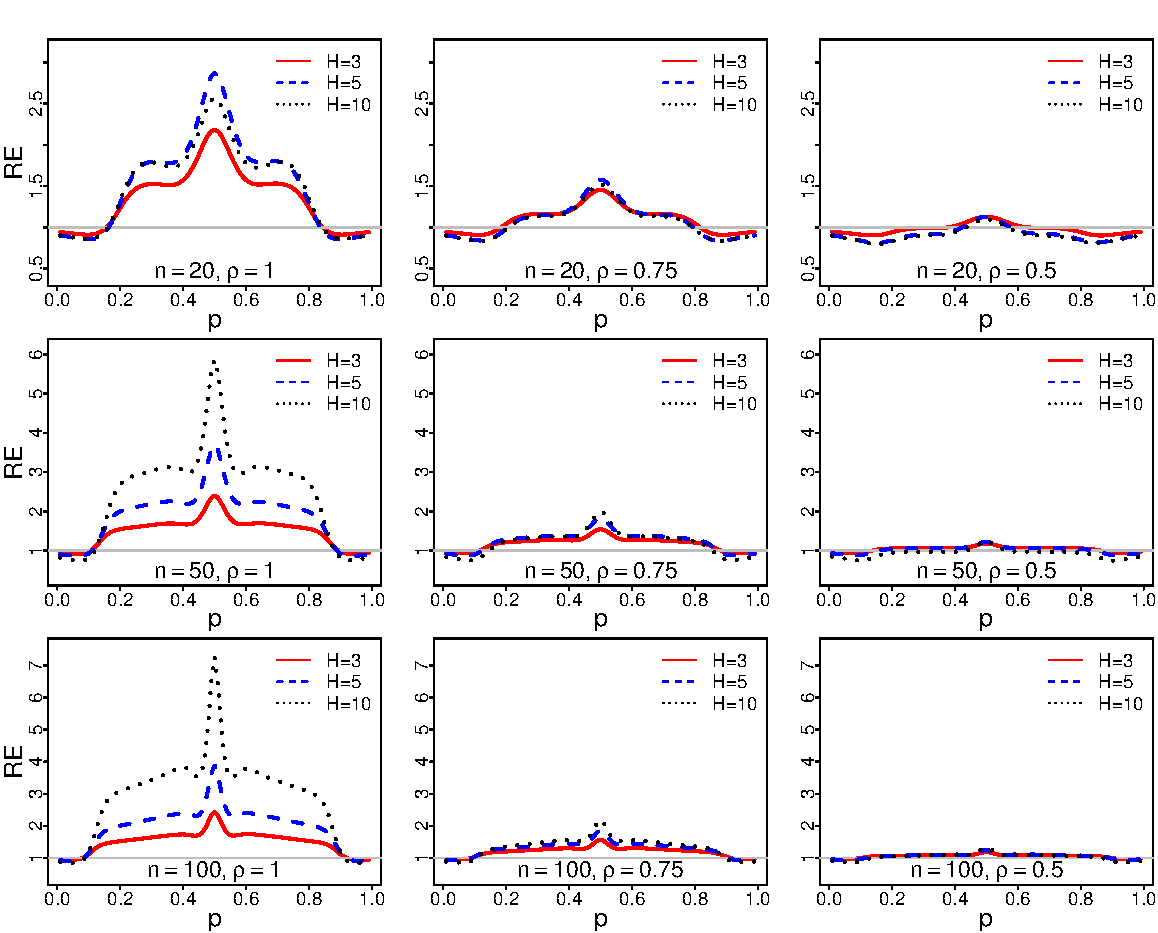
\includegraphics[scale=0.8]{Images/jps_ker_2-eps-converted-to.pdf}
\caption{\label{pic1}The simulated REs of $F_{n;srs}^k(.)$  to $ F_{n;jps}^{k}(.)$  as a function of $p$,  for $n \in \{20, 50, 100\}$, when $H=3$ (represented by red and solid line), $H=5$ (represented by blue and dashed line), $H=10$ (represented by black and dotted line) and  $\rho \in \{1,0.75,0.5\}$ under $ U(-1,1)$  distribution.}
\end{center}
\end{figure} 
\begin{figure}[t]
\begin{center}
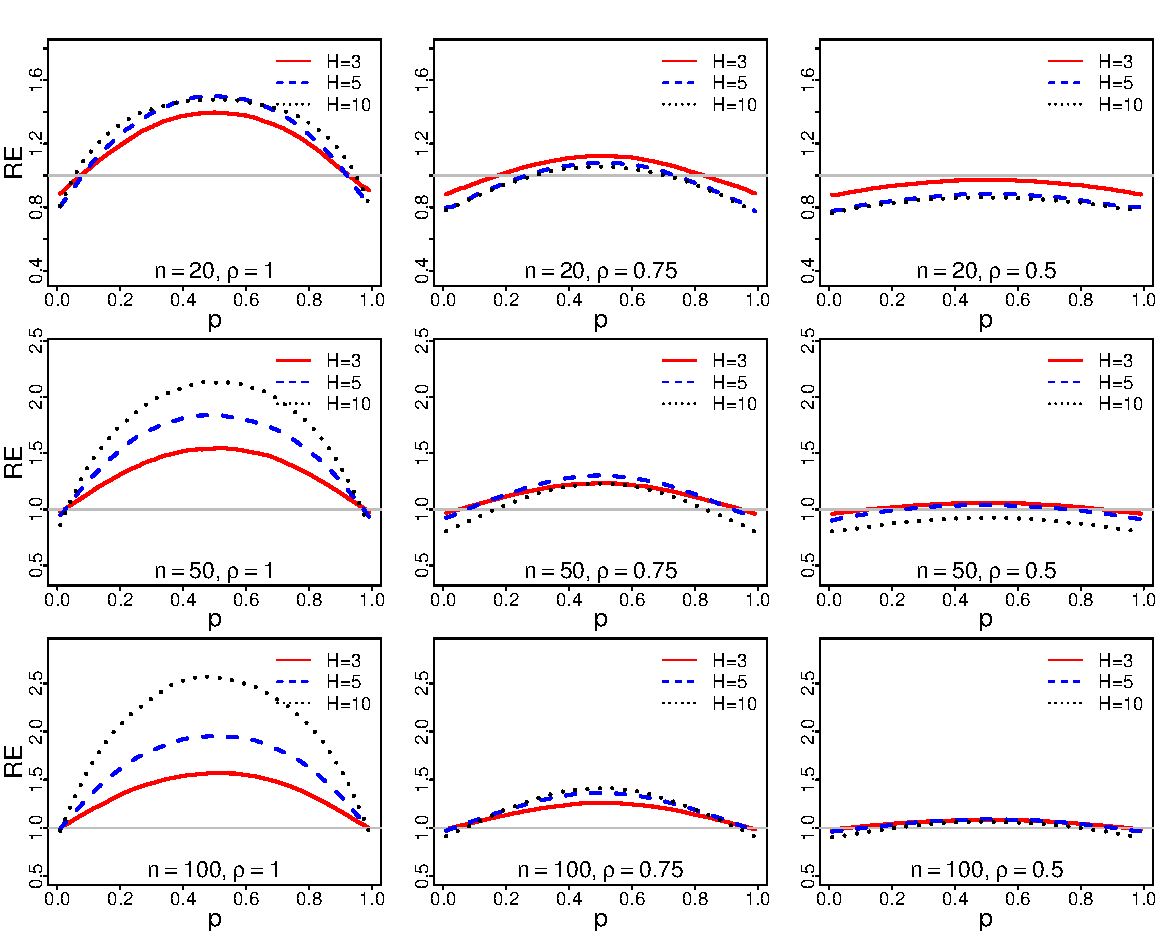
\includegraphics[scale=0.8]{Images/jps_edf_2-eps-converted-to.pdf}
\caption{\label{pic2}The simulated REs of $F_{n;srs}^*(.)$  to $ F_{n;jps}^{*}(.)$  as a function of $p$,  for $n \in \{20, 50, 100\}$, when $H=3$ (represented by red and solid line), $H=5$ (represented by blue and dashed line), $H=10$ (represented by black and dotted line) and  $\rho \in \{1,0.75,0.5\}$ under $ U(-1,1)$  distribution.}
\end{center}
\end{figure} 

\section{Monte Carlo Simulation}\label{Sec5}
To evaluate the  performance of the proposed KDF estimator, a Monte Carlo simulation study was carried out comparing the KDF estimator  under the JPS design with its counterpart based on SRS. The comparison was conducted under both perfect and imperfect ranking scenarios. Sample sizes of $n\in\{20,50,100\}$ and set sizes of $H\in\{3,5,10\}$ were considered throughout the study.

Imperfect ranking was generated using the linear ranking error model of   \cite{dell1972ranked}. In this framework, ranking is performed through an auxiliary variable $Y$ related to the study variable $X$ by
\[
Y=\rho\frac{X-\mu}{\sigma}+\sqrt{1-\rho^2}\,Z,
\]
where $\mu$ and $\sigma^2$ denote the mean and variance of $X$, respectively, and $Z$ is an independent standard normal random variable. The parameter $\rho$ determines the ranking quality, with larger values corresponding to more accurate rankings. 
The values $\rho=1$,  $\rho=0.75$, and $\rho=0.5$ were selected to represent perfect,  moderate, and weak ranking, respectively.

The efficiency comparison was based on the relative efficiency (RE) measure, defined as
\[
RE(p)=
\frac{\mathrm{MSE}\!\left(F_{n;srs}^{k}(Q_p)\right)}
{\mathrm{MSE}\!\left(F_{n;jps}^{k}(Q_p)\right)},
\]
where $Q_p$ denotes the $p$-th quantile of the underlying distribution. Values of $RE(p)$ greater than one indicate that the JPS-based estimator outperforms its SRS analogue at the corresponding quantile.

\begin{figure}[t]
\begin{center}
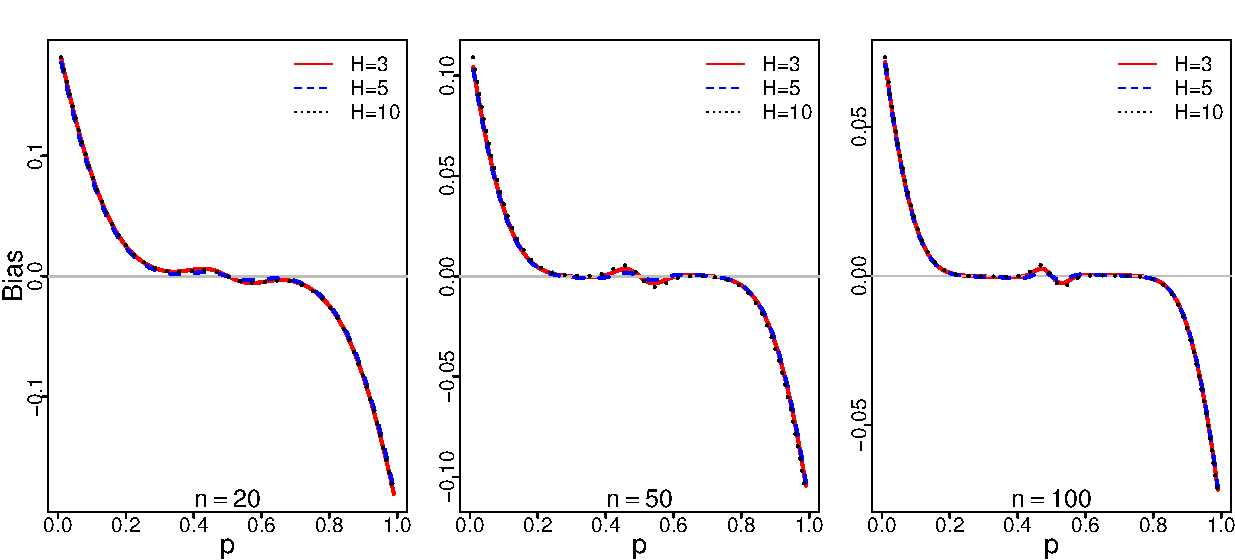
\includegraphics[scale=0.7]{Images/jps_ker_bias_3-eps-converted-to.pdf}
\caption{\label{pic3}The simulated biases of  $ F_{n;jps}^{k}(.)$  as a function of $p$,  for $n \in \{20, 50, 100\}$, when $H=3$ (represented by red and solid line), $H=5$ (represented by blue and dashed line), $H=10$ (represented by black and dotted line) and  $\rho = 1$ under $ U(-1,1)$  distribution.}
\end{center}
\end{figure} 
\begin{figure}[t]
\begin{center}
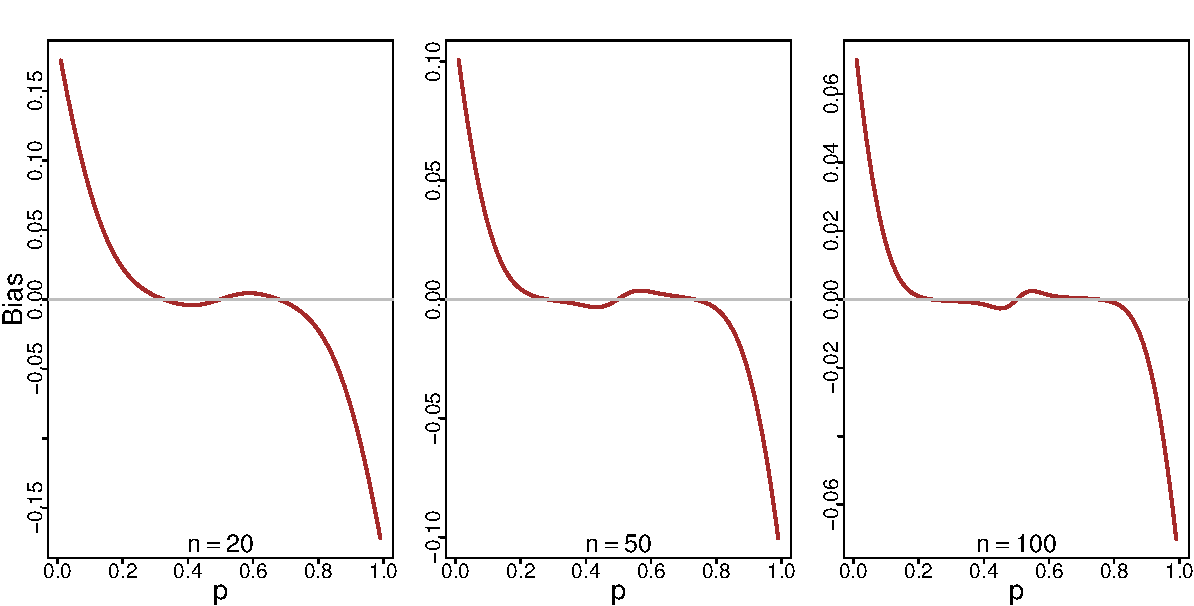
\includegraphics[scale=0.7]{Images/srs_ker_bias_2-eps-converted-to.pdf}
\caption{\label{pic4}The simulated biases of $F_{n;srs}^k(.)$   as a function of $p$,  for $n \in \{20, 50, 100\}$,  under $ U(-1,1)$  distribution.}
\end{center}
\end{figure} 
% The kernel function  utilized in the KDF estimators is truncated gaussian kernel function of the form  $k(x)=\frac{\phi(x)}{\Phi(4)-\Phi(-4)};\ \lvert x  \rvert \le 4,$   where the functions  $\phi(.)$ and $\Phi(.)$ represent the PDF and CDF of the standard normal distribution, respectively.
 
For each combination of $(n,H,\rho)$, 100{,}000 samples were generated from the uniform distribution on $(-1,1)$ under both sampling schemes, and the corresponding REs were computed for $p=0.01,0.02,\ldots,0.99$.
%Since preliminary investigations revealed that the choice of kernel function had a negligible impact on the relative efficiencies, only t
The KDF results based on the truncated Gaussian kernel are presented in Figure~\ref{pic1}.

From Figure \ref{pic1}, we find out that the REs are an increasing function of sample size $n$. The efficiency of the JPS estimators is usually higher around the center of the parent distribution and lower at its boundaries. Furthermore, the REs increase with the ranking quality $\rho$. 

Also, we observe that the optimal value of  the set size $H$, which leads to a higher efficiency,  depends on both ranking quality ($\rho$) and sample size ($n$). Specifically, a larger value of set size $H$ leads to a higher efficiency provided that the sample size is  large enough  and the ranking quality is sufficiently good. Therefore, small values for set sizes ($H=3, 5$) are recommended to be used in practice if the sample size is small or there is any doubt about ranking quality. 
The corresponding EDF results are also shown in Figure~\ref{pic2}, and their interpretation is similar to that of the KDF results.


It is well known that the EDF is an unbiased estimator of the CDF under both SRS and JPS sampling schemes.
 Therefore, in addition to comparing the MSEs, we investigated the finite-sample bias of the kernel-based CDF estimator under both SRS and JPS in the perfect ranking scenario. Since the theoretical bias of the estimator does not depend on the ranking quality, this investigation was conducted under the perfect ranking scenario.
 The results are shown in Figures   \ref{pic3} and \ref{pic4}. As expected from the theoretical results, similar patterns are observed under both the SRS and JPS sampling schemes.

We also observe that the magnitude of the bias decreases as the sample size increases across all considered scenarios. This behavior is consistent with theoretical expectations, since the bias of the kernel-based estimator diminishes as the bandwidth decreases with increasing sample size.

%The kernel-based estimator exhibits a small bias due to the smoothing procedure.
 The results indicate that the improvement in MSE achieved under JPS is not attributable to bias reduction. Rather, the gain arises primarily from variance reduction resulting from the additional ranking information incorporated into the JPS design. This advantage persists even when the ranking quality is imperfect, as JPS continues to provide a modest reduction in variability relative to SRS.
 
{\color{blue} Overall, these findings suggest that the practical advantage of JPS over SRS arises from utilizing the additional information provided by the ranked sample, which improves the precision of smooth CDF estimation for a given sample size.
}


%In this section, we conduct a comprehensive Monte Carlo simulation to compare the performance of the  KDF estimator based on SRS with its JPS sampling counterpart,  for both perfect and imperfect ranking set-ups.
% To this end, we have considered six different distributions as the parent distribution: standard normal distribution ($N(0,1)$), Student's t- distribution with $5$ degrees of freedom {\color{purple}$\left(t\left(5\right)\right)$}, standard Laplace distribution ($La(0,1)$), standard exponential distribution ($E(1)$), gamma distribution with scale parameter $1$ and shape parameter $0.5$ ($G(0.5, 1)$), and gamma distribution with scale parameter $1$ and shape parameter $2$ ($G(2, 1)$). Therefore, both distributions with support on the real numbers $\mathbb{R}$ and lifetime distributions with support on $\left(0,+\infty \right)$ are considered in our study.
%  In this simulation study, we set  $n \in \lbrace 10, 50, 300 \rbrace$, and $H \in \lbrace 3, 5, 10 \rbrace$.
  % Therefore, we can compare the performance of the estimators for small, moderate, and large values of sample/set size. We can also observe the effect of increasing sample size (set size) on the performance of the estimators while the set size (sample size) is being fixed. 

%To perform ranking in the JPS samples, we use the method utilized in the linear ranking error model by \citet{dell1972ranked}. 
%According to this method, the ranking process is done by an auxiliary variable $(Y)$ correlated with the variable of interest $(X)$ as
%$$Y=\rho \frac{(X-\mu)}{\sigma}+\sqrt{1-\rho^2}Z,$$
% where $\mu$ and $\sigma^2$ are the mean and variance of $X$, respectively, and   the random variable $Z$ is characterized by being independent of $X$, which itself follows a standard normal distribution.  Also, the user controls  quality of ranking by choosing the parameter $\rho\in[0,1]$, as the correlation coefficient between $X$ and $Y$. 
%    %Additionally, the correlation coefficient $\rho$, which ranges from 0 to 1, determines the degree of correlation between $X$ and $Y$ and influences the ranking quality.
  %  In this simulation study, we select $\rho=1$ for perfect ranking, $\rho=0.9$ for good ranking, $\rho=0.75$ for moderate ranking, and $\rho=0.5$ for weak ranking. 
%    The kernel function  utilized in the KDF estimators is truncated gaussian kernel function of the form  $k(x)=\frac{\phi(x)}{\Phi(4)-\Phi(-4)};\ \lvert x  \rvert \le 4,$   where the functions  $\phi(.)$ and $\Phi(.)$ represent the PDF and CDF of the standard normal distribution, respectively.
 
% The relative efficiency (RE) of $F_{n;srs}^k\left(t\right)$ with respect to $F_{n;jps}^k\left(t\right)$ is defined as the ratio of their MSEs, which can be expressed as follows
% $$RE(p)=\frac{MSE(F_{n;srs}^k\left(Q_p\right))}{MSE(F_{n;jps}^k\left(Q_p\right))},$$
% where $Q_p$ is the $p$th quantile of the parent distribution. It is clear that an $RE$ value larger than $1$ indicates an advantage of using  the JPS estimator instead of SRS one at the $p$th quantile of the parent distribution. 
%
%For each $\left(n, H, \rho \right)$, we have generated 100,000 random samples from the JPS and SRS designs and obtained $RE(p)$ for $p \in \{0.01,0.02, \ldots,0.99\} $. Here, we only present the results in Figures \ref{pic1}-\ref{pic6} for the epanechnikov kernel function, because we have observed that  the choice of kernel function does not have much effect on the RE of the estimators.
% 
%




%This section briefly describes how to write papers for the 18th Iranian Statistical Conference so that those interested in participating in this conference can easily format their papers according to the conference format.
% 
%The paper should be a maximum of 8 pages using XePersian software based on this format. Obviously, if the paper is not in the conference format or the number of pages exceeds 8, it will be returned. For consistency, use the default font (this font - without any changes to this file) or the Times New Roman font (and its bold version).
%\section{Second Section Title}
%This section includes topics related to the second section, and definitions, examples, lemmas, theorems, proofs, propositions, corollaries, remarks, and algorithms should be written as follows.
%%%%%%%%%%%%%%%%%%%%%%%% Definition %%%%%%%%%%%%%%%%%%%%%%%%%%%%%%%%%%%
%\begin{dfn}\label{df1}
%This is a definition.
%\end{dfn}
%%%%%%%%%%%%%%%%%%%%%%%% Example %%%%%%%%%%%%%%%%%%%%%%%%%%%%%%%%%%%
%\begin{eg}\label{ex1}
%This is an example.
%\end{eg} 
%%%%%%%%%%%%%%%%%%%%%%%% Lemma %%%%%%%%%%%%%%%%%%%%%%%%%%%%%%%%%%%
%\begin{lem}\label{lm1}
%This is a lemma.
%\end{lem}
%%%%%%%%%%%%%%%%%%%%%%%% Theorem and proof  %%%%%%%%%%%%%%%%%%%%%%%%%%%%%%%%%%%
%\begin{thm}\label{th1}
%This is a theorem.
%\end{thm}
%\begin{proof}
%This is a proof. 
%\end{proof}
%%%%%%%%%%%%%%%%%%%%%%%%  Proposition  %%%%%%%%%%%%%%%%%%%%%%%%%%%%%%%%%%%
%\begin{pro}\label{pr1}
%This is a proposition.
%\end{pro}
%%%%%%%%%%%%%%%%%%%%%%%% Corollary %%%%%%%%%%%%%%%%%%%%%%%%%%%%%%%%%%%
%\begin{cor}\label{cor1}
%This is a corollary.
%\end{cor}
%%%%%%%%%%%%%%%%%%%%%%%% Remark %%%%%%%%%%%%%%%%%%%%%%%%%%%%%%%%%%%
%\begin{rem}\label{rm1}
%You can refer to definition \ref{df1}, lemma \ref{lm1}, theorem \ref{th1}, proposition \ref{pr1}, and
%corollary \ref{cor1} in the text.
%\end{rem}
%%%%%%%%%%%%%%%%%%%%%%%% Algorithm %%%%%%%%%%%%%%%%%%%%%%%%%%%%%%%%%%%
%\begin{alg}\label{alg1}
%This algorithm has the following \footnote{Steps}steps:
%\begin{itemize}
%\item 
%Step 1
%\item
%Step 2
%\item
%Step 3
%\end{itemize}
%\end{alg}
%\section{Formulas}
%%%%%%%%%%%%%%%%%%%%%%%%%%%%%%%% Unnumbered formula %%%%%%%%%%%%%%%%%%%%%%%
%A sample unnumbered formula is given below:
%\begin{equation*}
%\max\limits_{x \in \mathbb{R}} \ f(x).
%\end{equation*}
%%%%%%%%%%%%%%%%%%%%%%%%%%%%%%%% Numbered formula %%%%%%%%%%%%%%%%%%%%%%%
%Here is a sample of a numbered formula: 
%\begin{equation}\label{eq1}
%G_F(x)=\frac{1}{B(\alpha,\beta)}\int_{0}^{F(x)} t^{\alpha-1}(1-t)^{\beta-1}\,dt, \qquad \alpha>0, \beta>0.
%\end{equation}
%Formula numbering should be based on sections, and only relationships that are referenced in the text should have numbers.
%Below is a multiline formula that is the derivative of equation \eqref{eq1}:
%\begin{align}
%g_F(x)&=\frac{d}{dx} G_F(x)\nonumber\\
%&=\frac{1}{B(\alpha,\beta)} f(x) \left(F(x)\right)^{\alpha -1} \left(\bar F(x)\right)^{\beta -1}.
%\end{align}
%\section{Tables and Figures}
%Below is a sample table. Table \ref{tab1} contains four rows and three columns.
%\begin{table}[h]
%\begin{center}
%\small
%\caption{Table title should be here.}\label{tab1}
%\begin{tabular}{|c|cc|}
%  \hline
%  Column One & Column Two & Column Three \\  \hline \hline
%  1 & 2 & 3 \\
%  4 & 5 & 6 \\
%  7 & 8 & 9 \\  \hline
%\end{tabular}
%\end{center}
%\end{table}\\
%%%%%%%%%%%%%%%%%%%%%%%%%%%%%%%% Figure %%%%%%%%%%%%%%%%%%%%%%%%%%%%%%%%%


%%\section{How to Cite References}
%%References must be cited in the text. \cite{Craik:2005}, \cite{Feller:1972}, \cite{Genest:Rivest:1993}, and \cite{LZ15} are some examples of English references.

%\begin{figure}[ht]
%\begin{center}
%
\includegraphics[width=7cm,height=6cm]{Images/Fig2-eps-converted-to.pdf}
%
\includegraphics[width=7cm,height=6cm]{Images/Fig1-eps-converted-to.pdf}\\
%\vspace{-0.2cm}
%\caption{\footnotesize{Figure caption should be placed here.}}\label{fig1}
%\end{center}
%\end{figure}

\section*{Discussion and Conclusion}   
%Judgment post stratification (JPS) sampling plan is a beneficial approach for situations in which allocating a judgment rank to a sample unit in a set is far easier/cheaper than   precisely  quantifying it.
In this paper, we reviewed the general class of estimators for the population CDF in the JPS framework, encompassing both the EDF and KDF.
% Furthermore, the finite-sample and asymptotic properties of these estimators are presented and discussed.
%We showed that they are  more efficient than their competitors in the simple random sampling (SRS), as long as the ranking quality is better than random guessing. We found the necessary and sufficient condition for the estimators to be asymptotically unbiased. Additionally, we studied the  Glivenko-Cantelli type convergence and  asymptotic normality for the estimators in this class, assuming the same condition holds.
%We next focused on the kernel distribution function (KDF) in the class.
We compared the performance of the EDF and KDF estimators under JPS sampling with their counterparts under SRS using Monte Carlo simulation.
  %This analysis involved investigating various combinations of sample size, set size, ranking quality, parent distribution, and kernel function.
 It was found that the JPS estimators outperforms its  SRS competitor in most of the considered cases. 
 
{\color{blue} Future research in this area may focus on extending smooth CDF estimation under JPS sampling to multivariate settings and developing adaptive bandwidth selection approaches. Such extensions could further improve the flexibility and applicability of smooth CDF estimation methods under ranked sampling designs.}

 %Investigating more flexible estimation frameworks under complex ranked sampling designs may provide further opportunities for methodological development.

 %Finally, we showed the applicability and efficiency of our introduced procedure in practice using a real dataset, where actual concomitant variables were used for the ranking process.

%To the best of our knowledge, this work was the first attempt to estimate the CDF using a kernel function based on the JPS sampling scheme. Therefore, there is still plenty of room for more research.  As an example, consider a parameter of interest denoted by $\theta$, which can be expressed as $\theta = g(F)$, where $g(.)$ represents a known function.
% One can think of estimating the parameter $\theta$ by replacing the CDF $F$ with an appropriate estimator from the discussed class, and establishing its statistical properties. Moreover, it was shown that the true CDF of the post strata often follows the constraint: $F_{[1]}\left(t\right)\geq\ldots  \geq F_{[H]}\left(t\right)$, for all $t\in \mathbb{R}$. However, this constraint may not hold for sample estimates. \cite{wang2012isotonized} improves the EDF in the JPS setting by imposing this limitation onto the estimation process. Therefore, another interesting topic for future research could be how to utilize this limitation to improve the performance of  the KDF in the JPS setting. These topics can be discussed in  future works.
%The conclusion of the article should be presented in a maximum of 3 or 4 lines.

%\section*{Acknowledgments}   
%If you wish to include acknowledgments, this section should appear before the references.
%%%%%%%%%%%%%%%%%%%%%%%% References %%%%%%%%%%%%%%%%%%%%%%%%%%%%%

\begin{thebibliography}{9}

%\bibitem[Alvandi and Hatefi, 2021]{alvandi2021estimation}
%Alvandi, A. and Hatefi, A. (2021).
%\newblock Estimation of ordinal population with multi-observer ranked set
%  samples using ties information.
%\newblock {\em Statistical Methods in Medical Research}, 30(8):1960--1975.
%
%\bibitem[Alvandi and Hatefi, 2023]{alvandi2023analysis}
%Alvandi, A. and Hatefi, A. (2023).
%\newblock Analysis of ordinal populations from judgment post-stratification.
%\newblock {\em Stats}, 6(3):812--838.

\bibitem[Azizi~Kouhanestani et~al., 2025]{kouhanestani2025statistical}
Azizi~Kouhanestani, M., Zamanzade, E., and Goli, S. (2025),
\newblock Statistical inference on the cumulative distribution function using
  judgment post stratification,
\newblock {\em Journal of Computational and Applied Mathematics}, 458:116340.

%\bibitem[Azzalini, 1981]{azzalini1981note}
%Azzalini, A. (1981),
%\newblock A note on the estimation of a distribution function and quantiles by
%  a kernel method,
%\newblock {\em Biometrika}, 68(1):326--328.

%\bibitem[{\c{C}}etin and Koyuncu, 2024]{ccetin2024new}
%{\c{C}}etin, A.~E. and Koyuncu, N. (2024).
%\newblock New robust class of estimators for population mean under different
%  sampling designs.
%\newblock {\em Journal of Computational and Applied Mathematics}, 441:115669.
%
%\bibitem[Chen et~al., 2018]{chen2018global}
%Chen, W., Tian, Y., and Xie, M. (2018).
%\newblock The global minimum variance unbiased estimator of the parameter for a
%  truncated parameter family under the optimal ranked set sampling.
%\newblock {\em Journal of Statistical Computation and Simulation},
%  88(17):3399--3414.
%
%\bibitem[Chen et~al., 2021]{chen2021pareto}
%Chen, W., Yang, R., Yao, D., and Long, C. (2021).
%\newblock Pareto parameters estimation using moving extremes ranked set
%  sampling.
%\newblock {\em Statistical Papers}, 62(3):1195--1211.

\bibitem[Dastbaravarde et~al., 2016]{dastbaravarde2016some}
Dastbaravarde, A., Arghami, N.~R., and Sarmad, M. (2016),
\newblock Some theoretical results concerning non parametric estimation by
  using a judgment poststratification sample,
\newblock {\em Communications in Statistics-Theory and Methods},
  45(8):2181--2203.

\bibitem[Dell and Clutter, 1972]{dell1972ranked}
Dell, T. and Clutter, J. (1972),
\newblock Ranked set sampling theory with order statistics background,
\newblock {\em Biometrics}, pages 545--555.
%
%\bibitem[Dizicheh et~al., 2021]{dizicheh2021efficient}
%Dizicheh, M.~A., Zamanzade, E., and Iranpanah, N. (2021).
%\newblock Efficient estimation of the odds using judgment post stratification.
%\newblock {\em Brazilian Journal of Probability and Statistics},
%  35(2):375--391.
%
%\bibitem[D{\"u}mbgen and Zamanzade, 2020]{dumbgen2020inference}
%D{\"u}mbgen, L. and Zamanzade, E. (2020).
%\newblock Inference on a distribution function from ranked set samples.
%\newblock {\em Annals of the Institute of Statistical Mathematics},
%  72(1):157--185.
%
%\bibitem[Eftekharian and Razmkhah, 2017]{eftekharian2017estimating}
%Eftekharian, A. and Razmkhah, M. (2017).
%\newblock On estimating the distribution function and odds using ranked set
%  sampling.
%\newblock {\em Statistics \& Probability Letters}, 122:1--10.
%
%\bibitem[Frey and Feeman, 2012]{frey2012improved}
%Frey, J. and Feeman, T.~G. (2012).
%\newblock An improved mean estimator for judgment post-stratification.
%\newblock {\em Computational Statistics \& Data Analysis}, 56(2):418--426.
%
%\bibitem[Frey and Feeman, 2013]{frey2013variance}
%Frey, J. and Feeman, T.~G. (2013).
%\newblock Variance estimation using judgment post-stratification.
%\newblock {\em Annals of the Institute of Statistical Mathematics},
%  65:551--569.
%
%\bibitem[Frey and Zhang, 2019a]{frey2019improved}
%Frey, J. and Zhang, Y. (2019a).
%\newblock Improved exact confidence intervals for a proportion using ranked-set
%  sampling.
%\newblock {\em Journal of the Korean Statistical Society}, 48:493--501.
%
%\bibitem[Frey and Zhang, 2019b]{frey2019omnibus}
%Frey, J. and Zhang, Y. (2019b).
%\newblock An omnibus two-sample test for ranked-set sampling data.
%\newblock {\em Journal of the Korean Statistical Society}, 48:106--116.
%
%\bibitem[Frey and Zhang, 2021]{frey2021robust}
%Frey, J. and Zhang, Y. (2021).
%\newblock Robust confidence intervals for a proportion using ranked-set
%  sampling.
%\newblock {\em Journal of the Korean Statistical Society}, 50:1009--1028.
%
\bibitem[Gulati, 2004]{gulati2004smooth}
Gulati, S. (2004),
\newblock Smooth non-parametric estimation of the distribution function from
  balanced ranked set samples,
\newblock {\em Environmetrics}, 15(5):529--539.

%\bibitem[He et~al., 2020]{he2020maximum}
%He, X., Chen, W., and Qian, W. (2020).
%\newblock Maximum likelihood estimators of the parameters of the log-logistic
%  distribution.
%\newblock {\em Statistical papers}, 61(5):1875--1892.
%
%\bibitem[He et~al., 2021]{he2021modified}
%He, X., Chen, W., and Yang, R. (2021).
%\newblock Modified best linear unbiased estimator of the shape parameter of
%  log-logistic distribution.
%\newblock {\em Journal of Statistical Computation and Simulation},
%  91(2):383--395.
%
%\bibitem[Koyuncu and Karag{\"o}z, 2021]{koyuncu2021designing}
%Koyuncu, N. and Karag{\"o}z, D. (2021).
%\newblock Designing robust modified r control charts for asymmetric
%  distributions under ranked set and median ranked set sampling.
%\newblock {\em Computational Statistics}, 36(2):1093--1121.

%\bibitem[MacEachern et~al., 2002]{maceachern2002new}
%MacEachern, S.~N., {\"O}zt{\"u}rk, {\"O}., Wolfe, D.~A., and Stark, G.~V.
%  (2002).
%\newblock A new ranked set sample estimator of variance.
%\newblock {\em Journal of the Royal Statistical Society: Series B (Statistical
%  Methodology)}, 64(2):177--188.

\bibitem[MacEachern et~al., 2004]{maceachern2004judgement}
MacEachern, S.~N., Stasny, E.~A., and Wolfe, D.~A. (2004),
\newblock Judgement post-stratification with imprecise rankings,
\newblock {\em Biometrics}, 60(1):207--215.

%\bibitem[Mahdizadeh and Zamanzade, 2017]{mahdizadeh2017reliability}
%Mahdizadeh, M. and Zamanzade, E. (2017).
%\newblock Reliability estimation in multistage ranked set sampling.
%\newblock {\em REVSTAT-Statistical Journal}, 15(4):565--581.
%
%\bibitem[Mahdizadeh and Zamanzade, 2018]{mahdizadeh2018interval}
%Mahdizadeh, M. and Zamanzade, E. (2018).
%\newblock Interval estimation of p (x< y) in ranked set sampling.
%\newblock {\em Computational Statistics}, 33(3):1325--1348.
%
%\bibitem[Mahdizadeh and Zamanzade, 2021]{mahdizadeh2021smooth}
%Mahdizadeh, M. and Zamanzade, E. (2021).
%\newblock Smooth estimation of the area under the roc curve in multistage
%  ranked set sampling.
%\newblock {\em Statistical Papers}, 62(4):1753--1776.
%
%\bibitem[McIntyre, 1952]{mcintyre1952method}
%McIntyre, G. (1952).
%\newblock A method for unbiased selective sampling, using ranked sets.
%\newblock {\em Australian journal of agricultural research}, 3(4):385--390.
%
%\bibitem[Moon et~al., 2020]{moon2020empirical}
%Moon, C., Wang, X., and Lim, J. (2020).
%\newblock Empirical likelihood inference for area under the roc curve using
%  ranked set samples.
%\newblock {\em arXiv preprint arXiv:2010.12185}.
%
%\bibitem[Nadaraya, 1964]{nadaraya1964some}
%Nadaraya, E.~A. (1964).
%\newblock Some new estimates for distribution functions.
%\newblock {\em Theory of Probability \& Its Applications}, 9(3):497--500.
%
%\bibitem[Newer, 2024]{newer2024prediction}
%Newer, H.~A. (2024).
%\newblock Prediction of future observations based on ordered extreme k-records
%  ranked set sampling with unequal fixed and random sample sizes.
%\newblock {\em Journal of Computational and Applied Mathematics}, 445:115798.
%
%\bibitem[Omidvar et~al., 2018]{omidvar2018judgment}
%Omidvar, S., Jafari~Jozani, M., and Nematollahi, N. (2018).
%\newblock Judgment post-stratification in finite mixture modeling: An example
%  in estimating the prevalence of osteoporosis.
%\newblock {\em Statistics in medicine}, 37(30):4823--4836.
%
%\bibitem[Ozturk, 2012]{ozturk2012combining}
%Ozturk, O. (2012).
%\newblock Combining ranking information in judgment post stratified and ranked
%  set sampling designs.
%\newblock {\em Environmental and ecological statistics}, 19(1):73--93.
%
%\bibitem[Ozturk, 2015]{ozturk2015statistical}
%Ozturk, O. (2015).
%\newblock Statistical inference for population quantiles and variance in
%  judgment post-stratified samples.
%\newblock {\em Quality control and applied statistics}, 60(3):217--218.
%
%\bibitem[Ozturk and Kravchuk, 2021]{ozturk2021judgment}
%Ozturk, O. and Kravchuk, O. (2021).
%\newblock Judgment post-stratified assessment combining ranking information
%  from multiple sources, with a field phenotyping example.
%\newblock {\em Journal of Agricultural, Biological and Environmental
%  Statistics}, 26(3):329--348.

\bibitem[Presnell and Bohn, 1999]{presnell1999u}
Presnell, B. and Bohn, L.~L. (1999),
\newblock U-statistics and imperfect ranking in ranked set sampling,
\newblock {\em Journal of Nonparametric Statistics}, 10(2):111--126.
%
%\bibitem[Qian et~al., 2021]{qian2021parameter}
%Qian, W., Chen, W., and He, X. (2021).
%\newblock Parameter estimation for the pareto distribution based on ranked set
%  sampling.
%\newblock {\em Statistical papers}, 62(1):395--417.
%
%\bibitem[Rasheed et~al., 2024]{rasheed2024designing}
%Rasheed, Z., Zhang, H., Anwar, S.~M., Noor-ul Amin, M., Adegoke, N.~A., and
%  Abbasi, S.~A. (2024).
%\newblock Designing efficient dispersion control charts under various
%  ranked-set sampling approaches.
%\newblock {\em Journal of Computational and Applied Mathematics}, 441:115680.

%\bibitem[Silverman, 2018]{silverman2018density}
%Silverman, B.~W. (2018),
%\newblock {\em Density estimation for statistics and data analysis},
%\newblock Routledge.
%
%\bibitem[Stokes, 1980]{stokes1980estimation}
%Stokes, S.~L. (1980).
%\newblock Estimation of variance using judgment ordered ranked set samples.
%\newblock {\em Biometrics}, pages 35--42.
%
%\bibitem[Stokes and Sager, 1988]{stokes1988characterization}
%Stokes, S.~L. and Sager, T.~W. (1988).
%\newblock Characterization of a ranked-set sample with application to
%  estimating distribution functions.
%\newblock {\em Journal of the American Statistical Association},
%  83(402):374--381.
%
%\bibitem[Takahasi and Wakimoto, 1968]{takahasi1968unbiased}
%Takahasi, K. and Wakimoto, K. (1968).
%\newblock On unbiased estimates of the population mean based on the sample
%  stratified by means of ordering.
%\newblock {\em Annals of the institute of statistical mathematics},
%  20(1):1--31.
%
%\bibitem[Wang et~al., 2024]{wang2024fisher}
%Wang, S., Chen, W., and Yang, R. (2024).
%\newblock Fisher information in ranked set sampling from the simple linear
%  regression model.
%\newblock {\em Communications in Statistics-Simulation and Computation},
%  53(3):1274--1284.
%
%\bibitem[Wang et~al., 2008]{wang2008nonparametric}
%Wang, X., Lim, J., and Stokes, L. (2008).
%\newblock A nonparametric mean estimator for judgment poststratified data.
%\newblock {\em Biometrics}, 64(2):355--363.
%
%\bibitem[Wang et~al., 2012]{wang2012isotonized}
%Wang, X., Wang, K., and Lim, J. (2012).
%\newblock Isotonized cdf estimation from judgment poststratification data with
%  empty strata.
%\newblock {\em Biometrics}, 68(1):194--202.
%
%\bibitem[Watson and Leadbetter, 1964]{watson1964hazard}
%Watson, G.~S. and Leadbetter, M. (1964).
%\newblock Hazard analysis ii.
%\newblock {\em Sankhy{\=a}: The Indian Journal of Statistics, Series A}, pages
%  101--116.
%
%\bibitem[Winter, 1973]{winter1973strong}
%Winter, B. (1973).
%\newblock Strong uniform consistency of integrals of density estimators.
%\newblock {\em Canadian Journal of Statistics}, 1(1-2):247--253.
%
%\bibitem[Woodall et~al., 2024]{woodall2024reevaluating}
%Woodall, W.~H., Haq, A., Mahmoud, M.~A., and Saleh, N.~A. (2024).
%\newblock Reevaluating the performance of control charts based on ranked-set
%  sampling.
%\newblock {\em Quality Engineering}, 36(2):365--370.

\bibitem[Yamato, 1973]{yamato1973uniform}
Yamato, H. (1973),
\newblock Uniform convergence of an estimator of a distribution function,
\newblock {\em Bulletin of Mathematical Statistics}, 15:69--78.
%%
%\bibitem[Zamanzade, 2016]{zamanzade2016isotonized}
%Zamanzade, E. (2016).
%\newblock An isotonized variance estimator for judgment post stratified data.
%\newblock {\em Journal of the Korean Statistical Society}, 45(1):25--32.
%
%\bibitem[Zamanzade et~al., 2020]{zamanzade2020efficient}
%Zamanzade, E., Mahdizadeh, M., and Samawi, H.~M. (2020).
%\newblock Efficient estimation of cumulative distribution function using moving
%  extreme ranked set sampling with application to reliability.
%\newblock {\em AStA Advances in Statistical Analysis}, 104(3):485--502.
%
%\bibitem[Zamanzade and Vock, 2018]{zamanzade2018some}
%Zamanzade, E. and Vock, M. (2018).
%\newblock Some nonparametric tests of perfect judgment ranking for judgment
%  post stratification.
%\newblock {\em Statistical Papers}, 59(3):1085--1100.
%
%\bibitem[Zamanzade and Wang, 2017]{zamanzade2017estimation}
%Zamanzade, E. and Wang, X. (2017).
%\newblock Estimation of population proportion for judgment post-stratification.
%\newblock {\em Computational Statistics \& Data Analysis}, 112:257--269.


%\bibitem[Craik (2005)]{Craik:2005}
%Craik A.D.D. (2005), Prehistory of Fa\`{a} di Bruno's formula, {\it The American Mathematical Monthly} 112, 2,  119-130.
%\bibitem[Feller (1972)]{Feller:1972} 
%Feller W. (1972), {\it An introduction to probability theory and its applications,} New York, John Wiley.
%\bibitem[Genest and  Rivest (1993)]{Genest:Rivest:1993}
%Genest C. and  Rivest L.P. (1993), Statistical inference
%procedures for bivariate Archimedean copulas, {\it J. Amer.
%Statist. Assoc.} 88,  1034 - 1043.
%
%\bibitem[Li et al. (2015)]{LZ15}
%Li K., Zheng W. and Ai M. (2015), Optimal designs for the proportional interference model, {\it The Annals of Statistics}, 43(4), 1596-1616.
\end{thebibliography}
 \end{document}

